\hypertarget{IMRPhenomD_8cpp}{}\section{src/\+I\+M\+R\+PhenomD.cpp File Reference}
\label{IMRPhenomD_8cpp}\index{src/\+I\+M\+R\+Phenom\+D.\+cpp@{src/\+I\+M\+R\+Phenom\+D.\+cpp}}
{\ttfamily \#include \char`\"{}I\+M\+R\+Phenom\+D.\+h\char`\"{}}\newline
{\ttfamily \#include \char`\"{}util.\+h\char`\"{}}\newline
{\ttfamily \#include $<$math.\+h$>$}\newline
{\ttfamily \#include $<$iostream$>$}\newline
{\ttfamily \#include $<$complex.\+h$>$}\newline
{\ttfamily \#include $<$cmath$>$}\newline
{\ttfamily \#include $<$adolc/adouble.\+h$>$}\newline
{\ttfamily \#include $<$adolc/taping.\+h$>$}\newline
{\ttfamily \#include $<$adolc/drivers/drivers.\+h$>$}\newline
{\ttfamily \#include $<$typeinfo$>$}\newline
Include dependency graph for I\+M\+R\+Phenom\+D.\+cpp\+:\nopagebreak
\begin{figure}[H]
\begin{center}
\leavevmode
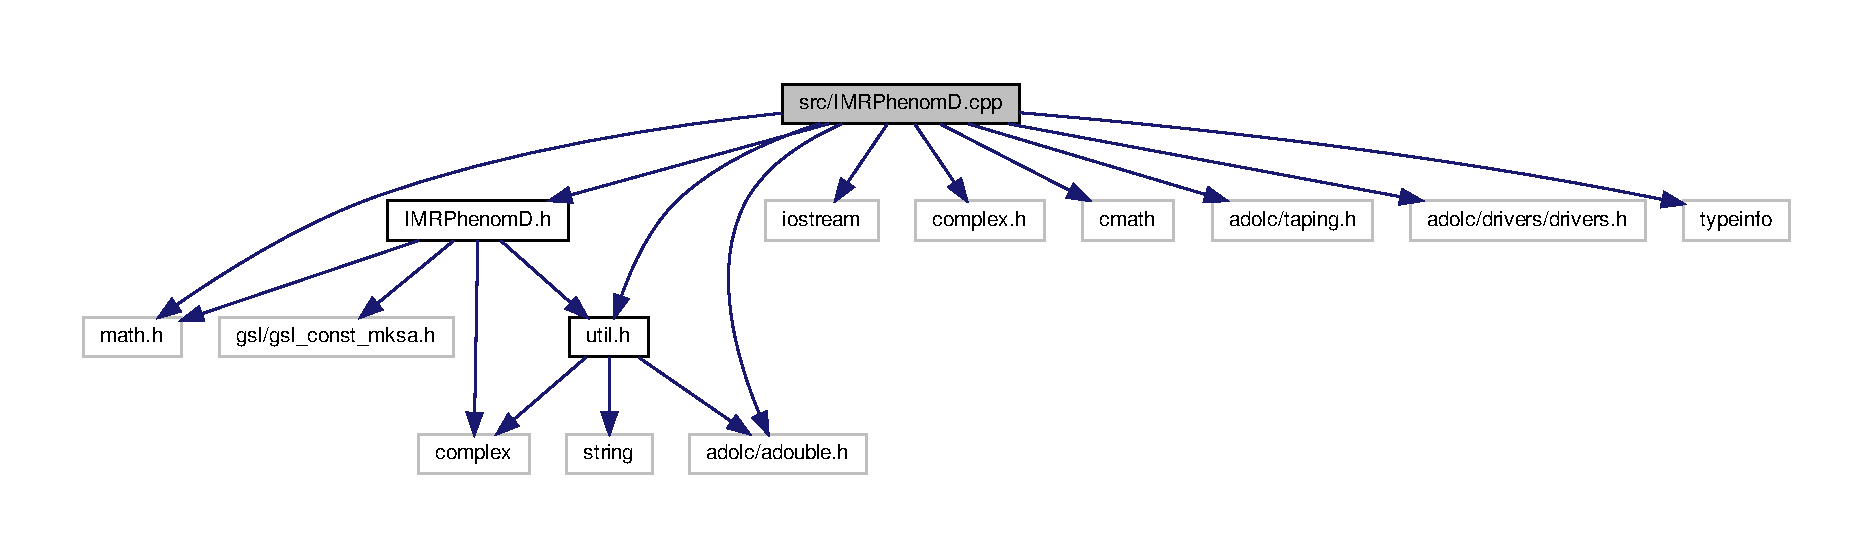
\includegraphics[width=350pt]{IMRPhenomD_8cpp__incl}
\end{center}
\end{figure}


\subsection{Detailed Description}
File that includes all the low level functions that go into constructing the waveform 